\section{Graphing Exponential Functions}

In this section, you will:
\begin{enumerate}
    \item examine properties of exponential functions
    \item examine graphs of exponential functions
\end{enumerate}


An exponential function can be written in forms \(f(x) = ab^x = a(1 + r)^x = ae^{kx}\):
\begin{itemize}
    \item \(a\) is the initial value because \(f(0) = a\).
    \item In the growth and decay models that we examine in this finite math textbook, \(a > 0\).
    \item \(b\) is often called the growth factor. We restrict \(b\) to be positive (\(b > 0\)) because even roots of negative numbers are undefined. We want the function to be defined for all values of \(x\), but \(b^x\) would be undefined for some values of \(x\) if \(b<0\).
    \item \(r\) is called the growth or decay rate. In the formula for the functions, we use \(r\) in decimal form, but in the context of a problem we usually state \(r\) as a percent.
    \item \(k\) is called the continuous growth rate or continuous decay rate.
\end{itemize}

\subsection{Properties of Exponential Growth Functions}

\begin{itemize}
    \item The function \(y = f(x) = ab^x\) represents growth if \(b > 1\) and \(a > 0\).
    \item The growth rate \(r\) is positive when \(b>1\). Because \(b = 1 + r > 1\), then \(r = b - 1 > 0\).
    \item The function \(y = f(x) = ae^{kx}\) represents growth if \(k > 0\) and \(a > 0\).
    \item The function is an increasing function; \(y\) increases as \(x\) increases.
\end{itemize}

\begin{center}
    \begin{tikzpicture}[scale=1, transform shape]
        % Axes
        \draw[->] (-3,0) -- (3,0) node[right] {$x$};
        \draw[->] (0,-1) -- (0,4) node[above] {$y$};

        % Exponential curve
        \draw[domain=-3:2, smooth, variable=\x, thick] plot ({\x}, {0.5*exp(\x)});

        % Point (0,a)
        \node[label={above:$(0,a)$}] at (0,0.5) {};

        % Labels for the equation (placed at top right)
        \node[align=left] at (-3,2) {
            $y = ab^x = a(1+r)^x = ae^{kx}$\\
            $a>0$\\
            $b>1, r>0, k>0$
        };

    \end{tikzpicture}
\end{center}

There are some properties the reader should notice:
\begin{itemize}
    \item \textbf{Domain:} All real numbers can be input to an exponential function. Mathematicians would write $\{x \in \mathbb{R}\}$ or simply $\mathbb{R}$.
    \item \textbf{Range:} If $a>0$, the range is the set of all positive real numbers. Mathematicians would write $\{x \in \mathbb{R}: x>0\}$.
    \item The graph is always above the $x$ axis.
    \item \textbf{Horizontal Asymptote:} when $b > 1$, the horizontal asymptote is the negative $x$ axis, as $x$ becomes large negative. Using mathematical notation: as $x \to -\infty$, then $y \to 0$.
    \item The vertical intercept is the point $(0,a)$ on the $y$-axis.
    \item There is no horizontal intercept because the function does not cross the $x$-axis.
\end{itemize}

\subsection{Properties of Exponential Decay Functions}
\begin{itemize}
    \item The function $y=f(x) = ab^x$ represents decay if $0 < b < 1$ and $a > 0$.
    \item The growth rate $r$ is negative when $0 < b < 1$. Because $b = 1 + r < 1$, then $r = b - 1 < 0$.
    \item The function $y=f(x) = ae^{kx}$ represents decay if $k < 0$ and $a > 0$.
    \item The function is a decreasing function; $y$ decreases as $x$ increases.
    \item \textbf{Domain:} All real numbers can be input to an exponential function. Mathematicians would write $\{x \in \mathbb{R}\}$ or simply $\mathbb{R}$.
    \item \textbf{Range:} If $a>0$, the range is the set of all positive real numbers. Mathematicians would write $\{x \in \mathbb{R}: x>0\}$.
    \item \textbf{Horizontal Asymptote:} when $b < 1$, the horizontal asymptote is the positive $x$ axis as $x$ becomes large positive. Using mathematical notation: as $x \to \infty$, then $y \to 0$.
    \item The vertical intercept is the point $(0,a)$ on the $y$-axis. There is no horizontal intercept because the function does not cross the $x$-axis.
\end{itemize}

The graphs for exponential growth and decay functions are displayed in the figure \ref{figure_exponential_growth_vs_decay} below for comparison.

% TODO fix labeling of figure here...

\begin{figure}[ht]
    \centering
    % First image in a minipage
    \begin{minipage}{0.45\textwidth}
        \centering\label{figure_exponential_growth_vs_decay}
        \begin{center}
            \begin{tikzpicture}[scale=.85, transform shape]
                % Axes
                \draw[->] (-3,0) -- (3,0) node[right] {$x$};
                \draw[->] (0,-1) -- (0,4) node[above] {$y$};

                % Exponential curve
                \draw[domain=-3:2, smooth, variable=\x, thick] plot ({\x}, {0.5*exp(\x)});

                % Point (0,a)
                \node[label={above:$(0,a)$}] at (0,0.5) {};

                % Labels for the equation (placed at top right)
                \node[align=left] at (-2.5,2) {
                    $y = ab^x = a(1+r)^x = ae^{kx}$\\
                    $a>0$\\
                    $b>1, r>0, k>0$
                };

            \end{tikzpicture}
        \end{center}
        \caption{Exponential Growth}
    \end{minipage}
    \hfill % Spacing between the figures
    % Second image in a minipage
    \begin{minipage}{0.45\textwidth}
        \centering
        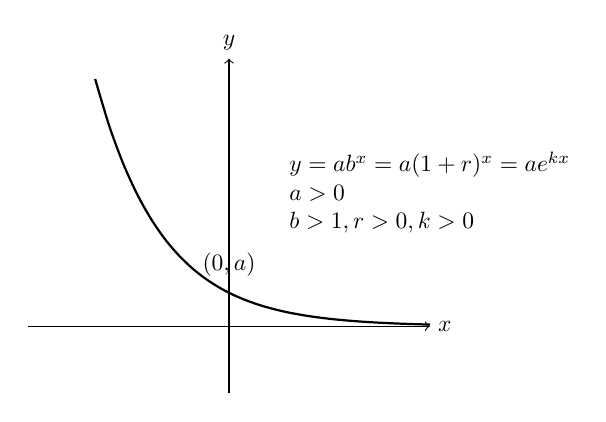
\begin{tikzpicture}[scale=.85, transform shape]
            % Axes
            \draw[->] (-3,0) -- (3,0) node[right] {$x$};
            \draw[->] (0,-1) -- (0,4) node[above] {$y$};

            % Exponential curve
            \draw[domain=-2:3, smooth, variable=\x, thick] plot ({\x}, {0.5*exp(-\x)});

            % Point (0,a)
            \node[label={above:$(0,a)$}] at (0,0.5) {};

            % Labels for the equation (placed at top right)
            \node[align=left] at (3,2) {
                $y = ab^x = a(1+r)^x = ae^{kx}$\\
                $a>0$\\
                $b>1, r>0, k>0$
            };

        \end{tikzpicture}
        \caption{Exponential Decay}
    \end{minipage}
\end{figure}

\subsection{An Exponential Function Is a One-to-One Function}

Observe that in the graph of an exponential function, each \( y \) value on the graph occurs only once. Therefore, every \( y \) value in the range corresponds to only one \( x \) value. So, for any particular value of \( y \), you can use the graph to see which value of \( x \) is the input to produce that \( y \) value as output. This property is called "one-to-one".

Because for each value of the output \( y \), you can uniquely determine the value of the corresponding input \( x \), thus every exponential function has an inverse function. The inverse function of an exponential function is a logarithmic function, which we will investigate in the next section.

\begin{example}
    $x$ years after the year \the\numexpr\year+1\relax, the population of the city of Fulton is given by the function $y=f(x) = 35000(1.03^x)$, and $x$ years after the year \the\numexpr\year+1\relax, the population of the city of Greenville is given by the function $y = g(x) = 80000(0.95^x)$. Compare the graphs of these functions.
\end{example}

\begin{solution}
    Here are graphs:

    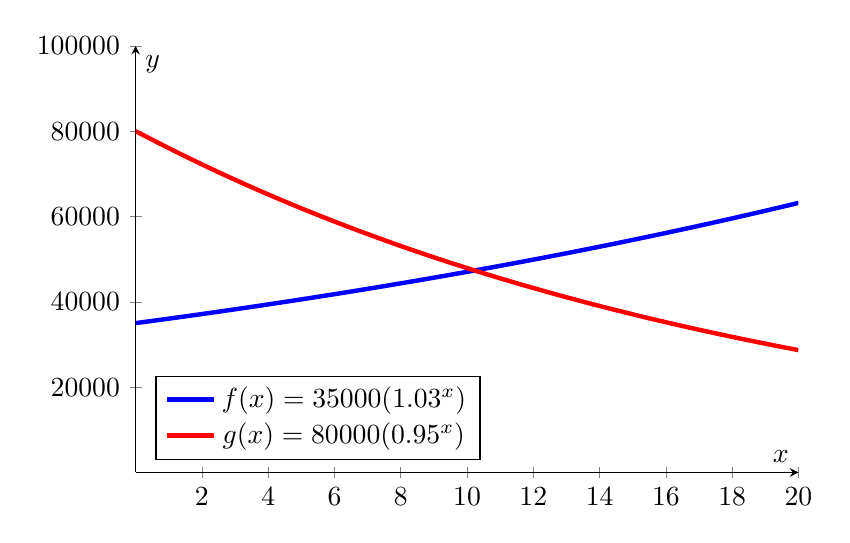
\begin{tikzpicture}
        \begin{axis}[
                axis lines=middle,
                xmin=0, xmax=20,
                ymin=0, ymax=100000,
                xlabel={$x$},
                ylabel={$y$},
                % title={Plot of the functions $f(x) = 35000(1.03^x)$ and $g(x) = 80000(0.95^x)$},
                legend pos=south west,
                % grid=both,
                % grid style={line width=.1pt, draw=gray!10},
                % major grid style={line width=.2pt,draw=gray!50},
                % scale only axis,
                width=10cm,
                height=7cm,
                yticklabel style={/pgf/number format/fixed, /pgf/number format/1000 sep=}, % format y ticks in fixed point notation
                scaled ticks=false % prevent pgfplots from scaling ticks into scientific notation
            ]

            % Plot f(x) = 35000(1.03^x)
            \addplot[domain=0:20, samples=100, blue, ultra thick] {35000*(1.03^x)};
            \addlegendentry{$f(x) = 35000(1.03^x)$}

            % Plot g(x) = 80000(0.95^x)
            \addplot[domain=0:20, samples=100, red, ultra thick] {80000*(0.95^x)};
            \addlegendentry{$g(x) = 80000(0.95^x)$}

        \end{axis}
    \end{tikzpicture}

    Some observations we may make:
    \begin{itemize}
        \item Fulton’s population is undergoing Exponential Growth.
              \begin{itemize}
                  \item $b = 1.03 >1$ and $r = 0.03 > 0$
                  \item The population is increasing.
              \end{itemize}
        \item Greenville’s population is undergoing Exponential Decay.
              \begin{itemize}
                  \item $b = 0.95 < 1$ and $r = -0.05 < 0$
                  \item The population is decreasing.
              \end{itemize}
        \item The initial population of Fulton in $\the\numexpr\year+1\relax$ is 35000.
        \item The initial population of Greenville in $\the\numexpr\year+1\relax$ is 80000.
        \item In general, the domains of both functions $f(x)$ and $g(x)$ are all real numbers, but realistically the populations of Fulton and Greenville cannot follow this model for all such values of $x$. Depending on how they were created, the models may be good enough for use for $x$ representing several years in the past to several years in the future.
        \item If the model holds, the populations of the two cities will be approximately equal sometime around $\the\numexpr\year+11\relax$.
    \end{itemize}

\end{solution}